

\tikzset{every picture/.style={line width=0.75pt}} %set default line width to 0.75pt        

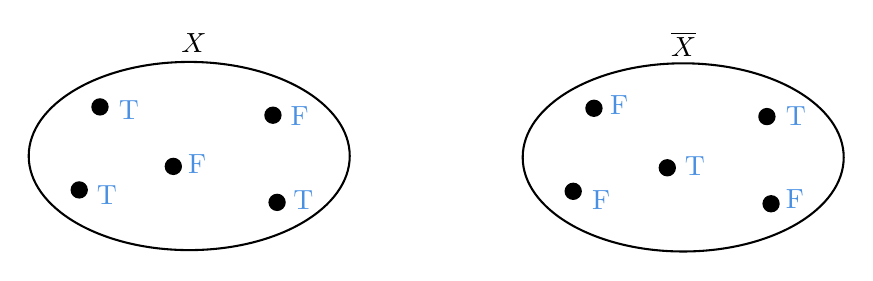
\begin{tikzpicture}[x=0.5pt,y=0.5pt,yscale=-1,xscale=1]
%uncomment if require: \path (0,300); %set diagram left start at 0, and has height of 300

%Shape: Ellipse [id:dp83662970590991] 
\draw   (8,96) .. controls (8,58.44) and (59.93,28) .. (124,28) .. controls (188.07,28) and (240,58.44) .. (240,96) .. controls (240,133.56) and (188.07,164) .. (124,164) .. controls (59.93,164) and (8,133.56) .. (8,96) -- cycle ;
%Shape: Circle [id:dp21341271480775648] 
\draw  [fill={rgb, 255:red, 0; green, 0; blue, 0 }  ,fill opacity=1 ] (54,60.5) .. controls (54,57.46) and (56.46,55) .. (59.5,55) .. controls (62.54,55) and (65,57.46) .. (65,60.5) .. controls (65,63.54) and (62.54,66) .. (59.5,66) .. controls (56.46,66) and (54,63.54) .. (54,60.5) -- cycle ;
%Shape: Circle [id:dp9929729618619046] 
\draw  [fill={rgb, 255:red, 0; green, 0; blue, 0 }  ,fill opacity=1 ] (39,120.5) .. controls (39,117.46) and (41.46,115) .. (44.5,115) .. controls (47.54,115) and (50,117.46) .. (50,120.5) .. controls (50,123.54) and (47.54,126) .. (44.5,126) .. controls (41.46,126) and (39,123.54) .. (39,120.5) -- cycle ;
%Shape: Circle [id:dp9620303268103491] 
\draw  [fill={rgb, 255:red, 0; green, 0; blue, 0 }  ,fill opacity=1 ] (107,103.5) .. controls (107,100.46) and (109.46,98) .. (112.5,98) .. controls (115.54,98) and (118,100.46) .. (118,103.5) .. controls (118,106.54) and (115.54,109) .. (112.5,109) .. controls (109.46,109) and (107,106.54) .. (107,103.5) -- cycle ;
%Shape: Circle [id:dp41706992941659915] 
\draw  [fill={rgb, 255:red, 0; green, 0; blue, 0 }  ,fill opacity=1 ] (179,66.5) .. controls (179,63.46) and (181.46,61) .. (184.5,61) .. controls (187.54,61) and (190,63.46) .. (190,66.5) .. controls (190,69.54) and (187.54,72) .. (184.5,72) .. controls (181.46,72) and (179,69.54) .. (179,66.5) -- cycle ;
%Shape: Circle [id:dp3550007068634743] 
\draw  [fill={rgb, 255:red, 0; green, 0; blue, 0 }  ,fill opacity=1 ] (182,129.5) .. controls (182,126.46) and (184.46,124) .. (187.5,124) .. controls (190.54,124) and (193,126.46) .. (193,129.5) .. controls (193,132.54) and (190.54,135) .. (187.5,135) .. controls (184.46,135) and (182,132.54) .. (182,129.5) -- cycle ;
%Shape: Ellipse [id:dp7490220245457752] 
\draw   (365,97) .. controls (365,59.44) and (416.93,29) .. (481,29) .. controls (545.07,29) and (597,59.44) .. (597,97) .. controls (597,134.56) and (545.07,165) .. (481,165) .. controls (416.93,165) and (365,134.56) .. (365,97) -- cycle ;
%Shape: Circle [id:dp3244374133914285] 
\draw  [fill={rgb, 255:red, 0; green, 0; blue, 0 }  ,fill opacity=1 ] (411,61.5) .. controls (411,58.46) and (413.46,56) .. (416.5,56) .. controls (419.54,56) and (422,58.46) .. (422,61.5) .. controls (422,64.54) and (419.54,67) .. (416.5,67) .. controls (413.46,67) and (411,64.54) .. (411,61.5) -- cycle ;
%Shape: Circle [id:dp41954634695015547] 
\draw  [fill={rgb, 255:red, 0; green, 0; blue, 0 }  ,fill opacity=1 ] (396,121.5) .. controls (396,118.46) and (398.46,116) .. (401.5,116) .. controls (404.54,116) and (407,118.46) .. (407,121.5) .. controls (407,124.54) and (404.54,127) .. (401.5,127) .. controls (398.46,127) and (396,124.54) .. (396,121.5) -- cycle ;
%Shape: Circle [id:dp7290812606891363] 
\draw  [fill={rgb, 255:red, 0; green, 0; blue, 0 }  ,fill opacity=1 ] (464,104.5) .. controls (464,101.46) and (466.46,99) .. (469.5,99) .. controls (472.54,99) and (475,101.46) .. (475,104.5) .. controls (475,107.54) and (472.54,110) .. (469.5,110) .. controls (466.46,110) and (464,107.54) .. (464,104.5) -- cycle ;
%Shape: Circle [id:dp4565505523195048] 
\draw  [fill={rgb, 255:red, 0; green, 0; blue, 0 }  ,fill opacity=1 ] (536,67.5) .. controls (536,64.46) and (538.46,62) .. (541.5,62) .. controls (544.54,62) and (547,64.46) .. (547,67.5) .. controls (547,70.54) and (544.54,73) .. (541.5,73) .. controls (538.46,73) and (536,70.54) .. (536,67.5) -- cycle ;
%Shape: Circle [id:dp8662075700047863] 
\draw  [fill={rgb, 255:red, 0; green, 0; blue, 0 }  ,fill opacity=1 ] (539,130.5) .. controls (539,127.46) and (541.46,125) .. (544.5,125) .. controls (547.54,125) and (550,127.46) .. (550,130.5) .. controls (550,133.54) and (547.54,136) .. (544.5,136) .. controls (541.46,136) and (539,133.54) .. (539,130.5) -- cycle ;

% Text Node
\draw (116,5) node [anchor=north west][inner sep=0.75pt]   [align=left] {$\displaystyle X$};
% Text Node
\draw (470,4) node [anchor=north west][inner sep=0.75pt]   [align=left] {$\displaystyle \overline{X}$};
% Text Node
\draw (71,54) node [anchor=north west][inner sep=0.75pt]  [color={rgb, 255:red, 74; green, 144; blue, 226 }  ,opacity=1 ] [align=left] {T};
% Text Node
\draw (121,93) node [anchor=north west][inner sep=0.75pt]  [color={rgb, 255:red, 74; green, 144; blue, 226 }  ,opacity=1 ] [align=left] {F};
% Text Node
\draw (426,50) node [anchor=north west][inner sep=0.75pt]  [color={rgb, 255:red, 74; green, 144; blue, 226 }  ,opacity=1 ] [align=left] {F};
% Text Node
\draw (553,118) node [anchor=north west][inner sep=0.75pt]  [color={rgb, 255:red, 74; green, 144; blue, 226 }  ,opacity=1 ] [align=left] {F};
% Text Node
\draw (195,58) node [anchor=north west][inner sep=0.75pt]  [color={rgb, 255:red, 74; green, 144; blue, 226 }  ,opacity=1 ] [align=left] {F};
% Text Node
\draw (413,119) node [anchor=north west][inner sep=0.75pt]  [color={rgb, 255:red, 74; green, 144; blue, 226 }  ,opacity=1 ] [align=left] {F};
% Text Node
\draw (55,115) node [anchor=north west][inner sep=0.75pt]  [color={rgb, 255:red, 74; green, 144; blue, 226 }  ,opacity=1 ] [align=left] {T};
% Text Node
\draw (197,119) node [anchor=north west][inner sep=0.75pt]  [color={rgb, 255:red, 74; green, 144; blue, 226 }  ,opacity=1 ] [align=left] {T};
% Text Node
\draw (480,94) node [anchor=north west][inner sep=0.75pt]  [color={rgb, 255:red, 74; green, 144; blue, 226 }  ,opacity=1 ] [align=left] {T};
% Text Node
\draw (553,58) node [anchor=north west][inner sep=0.75pt]  [color={rgb, 255:red, 74; green, 144; blue, 226 }  ,opacity=1 ] [align=left] {T};


\end{tikzpicture}

